%
% File eacl2017_supp.tex
%

\documentclass[11pt]{article}
\usepackage{colacl-onecolumn}
\usepackage{times}
\usepackage{url}
\usepackage{amsmath}
\usepackage{breqn}
\usepackage{latexsym}
\usepackage{pgfplotstable}
\usepackage{algorithm2e}
\usepackage{hhline}
\usepackage{multirow}
\usepackage{multicol}
\usepackage{caption}
\usepackage{subcaption}
%\usepackage{hyperref}
\usepackage{color}
\usepackage{lipsum,adjustbox}
\usepackage{tikz}
\usepackage{tikz-dependency}
\usepackage{rotating}
\usepackage{float}
\usepackage{xr}
\externaldocument[main:]{eacl2017}
\usetikzlibrary{shapes,fit,calc,er,positioning,intersections,decorations.shapes,mindmap,trees}
\tikzset{decorate sep/.style 2 args={decorate,decoration={shape backgrounds,shape=circle,
      shape size=#1,shape sep=#2}}}

\flushbottom \onecolumn

\newcommand{\parser}[1]{TUPA\textsubscript{#1}}
\newcommand{\secref}[1]{Section~\ref{#1}}
\newcommand{\figref}[1]{Figure~\ref{#1}}
\newcommand{\tabref}[1]{Table~\ref{#1}}
\DeclareMathOperator*{\argmin}{argmin}
\DeclareMathOperator*{\argmax}{argmax}
\SetKwRepeat{Do}{do}{while}

\makeatletter
\renewcommand{\paragraph}{
  \@startsection{paragraph}{4}
  {\z@}{.5ex \@plus .5ex \@minus .2ex}{-1em}
  {\normalfont\normalsize\bfseries}
}
\makeatother

\newcommand\BibTeX{B\textsc{ib}\TeX}

\title{Broad-Coverage Transition-Based UCCA Parsing \\
Supplementary Material}

\begin{document}
\maketitle



\section{Conversion Protocols for the Bilexical DAG and Tree Approximations}
\label{sec:conversion}

Here we describe the algorithms used in the conversion referred to in \secref{main:sec:exp_setup}
in the paper.

\paragraph{Notation.}
Let $L$ be the set of possible edge labels.
A UCCA graph over a sequence of tokens $w_1, \ldots, w_n$ is a directed acyclic graph
$G=(V,E, \ell)$, where $\ell:E\to L$ maps edges to labels.
For each token $w_i$ there exists a leaf (\emph{terminal}) $t_i \in V$.
A bilexical (dependency) graph over the same text consists of a set $A$ of
labeled dependency arcs $(t^\prime,l,t)$
between the terminals of $G$, where $t^\prime$ is the head, $t$ is the dependent and $l$ is
the edge label.

\paragraph{Conversion to bilexical graphs.}
Let $G=(V,E,\ell)$ be a UCCA graph with labels $\ell:E\rightarrow L$.
The conversion to a bilexical graph requires calculating the set $A$.
All non-terminals in $G$ are removed.

We define a linear order over possible edge labels $L$ (see \figref{fig:priority}).
For each node $u \in V$, denote by $h(u)$ its child with the highest-priority edge label.
Let $h^*(u)$ be the terminal reached by recursively applying $h(\cdot)$ over $u$.
For each terminal $t$, we define
\[
N(t) = \{(u,v)\in E \;|\; t=h^*(v) \wedge t \neq h^*(u) \}
\]
For each edge $(u,v)\in N(t)$, we add $h^*(u)$ as a head of $t$ in $A$,
with the label $\ell(u,v)$.
The complete conversion procedure to a bilexical graph is given in
Algorithm~\ref{alg:to_bilexical}\footnote{Note that this conversion procedure
is simpler than the head percolation procedure used for converting syntactic constituency
trees to dependency trees,
since $h(u)$ (similar to $u$'s head-containing child)
depends only on $\ell(h(u),u)$ and not on the sub-tree spanned by $u$,
because edge labels in UCCA directly express the role of the child in the parent unit, and
are thus sufficient for determining which of $u$'s children contains the head node.}.

\begin{algorithm}[h]
 \KwData{UCCA graph ${G}=(V,E,\ell)$}
 \KwResult{set $A$ of labeled bilexical arcs}
 $A \leftarrow \emptyset$\;
 \ForEach{$t \in \mathrm{Terminals}(V)$} {
  \ForEach{$(u,v)\in N(t)$} {
   $t^\prime \leftarrow h^*(u)$\;
   $A \leftarrow A \cup \{(t^\prime, \ell(u, v), t)\}$\;
  }
 }
 \caption{Conversion to bilexical graphs.}
 \label{alg:to_bilexical}
\end{algorithm}

\paragraph{Conversion from bilexical graphs.}
The inverse conversion introduces non-terminal nodes back into the graph.
As the distinction between low- and high-attaching nodes is lost in the
conversion, we assume that attachments are always
low-attaching.
Let $A$ be a the labeled arc set of a bilexical graph.
Iterating over the terminals in topological order according to $A$,
we add its members as terminals to graph
and create a pre-terminal parent $u_t$ for each terminal $t$,
with an edge labeled as \textit{Terminal} between them.
The parents of the pre-terminals are determined by the terminal's parent in the bilexical
graph: if $t^\prime$ is a head of $t$ in $A$, then $u_{t^\prime}$ will be a parent of $u_t$.
We add an intermediate node in between if $t$ has any dependents in $A$,
to allow adding their pre-terminals as children later.
Edge labels for the intermediate edges are determined by a rule-based function, denoted by
$\mathrm{Label}(t)$.
This procedure is given in Algorithm~\ref{alg:from_bilexical}.

\begin{algorithm}[h]
 \KwData{list $T$ of terminals, set $A$ of labeled bilexical arcs}
 \KwResult{UCCA graph $G=(V,E,\ell)$}
 \SetKwFunction{Label}{Label}{}{}
 $V \leftarrow \emptyset$\;
 $E \leftarrow \emptyset$\;
 \ForEach{$t \in \mathrm{TopologicalSort}(T, A)$} {
  $u_t \leftarrow \mathrm{Node()}$\;
  $V \leftarrow V \cup \{u_t, t\}$\;
  $E \leftarrow E \cup \{(u_t, t)\}$\;
  $\ell(u_t,t)\leftarrow\mathit{Terminal}$\;
  \ForEach{$t^\prime\in T,l\in L$} {
   \If{$(t^\prime,l,t)\in A$} {
    \eIf{$\exists t^{\prime\prime}\in T,l^\prime\in L : (t,l^\prime,t^{\prime\prime}) \in A$} {
     $u \leftarrow \mathrm{Node()}$\;
     $E \leftarrow E \cup \{(u, u_t)\}$\;
     $\ell(u, u_t) \leftarrow \Label(t)$\;
    } {
     $u \leftarrow u_t$\;
    }
    $E \leftarrow E \cup \{(u_{t^\prime}, u)\}$\;
    $\ell(u_{t^\prime}, u) \leftarrow l$\;
    }
  }
 }
 
  \SetKwProg{func}{Function}{}{}
  
  \func{\Label}{
  \KwData{node $t \in T$}
  \KwResult{label $l\in L$}

   \uIf{$\mathrm{IsPunctuation}(t)$}{
    \Return \textit{Punctuation}\;
   }
   \uElseIf{$\exists t^\prime \in T : (t,\textit{ParallelScene},t^\prime)\in A$}{
    \Return \textit{ParallelScene}\;
   }
   \uElseIf{$\exists t^\prime \in T : (t,\textit{Participant},t^\prime)\in A$}{
    \Return \textit{Process}\;
   }
   \uElse{
    \Return \textit{Center}\;
   }
  }
 \caption{Conversion from bilexical graphs.}
 \label{alg:from_bilexical}
\end{algorithm}

\begin{figure}[H]
\begin{multicols}{2}
\begin{enumerate}
\item $C$ (\textit{Center})
\item $N$ (\textit{Connector})
\item $H$ (\textit{ParallelScene})
\item $P$ \textit{Process})
\item $S$ (\textit{State})
\item $A$ (\textit{Participant})
\item $D$ (\textit{Adverbial})
\item $T$ (\textit{Time})
\item $E$ (\textit{Elaborator})
\item $R$ (\textit{Relator})
\item $F$ (\textit{Function})
\item $L$ (\textit{Linker})
\item $LR$ (\textit{LinkRelation})
\item $LA$ (\textit{LinkArgument})
\item $G$ (\textit{Ground})
\item $\mathit{Terminal}$ (\textit{Terminal})
\item $U$ (\textit{Punctuation})
\end{enumerate}
\end{multicols}
\caption{Priority order of edge labels, used in Algorithm~\ref{alg:to_bilexical}.}
\label{fig:priority}
\end{figure}

\paragraph{Conversion to trees.}

To convert a UCCA graph to a tree, we simply remove the remote edges.
Converting the sentence in \figref{main:fig:graduation} in the paper
results in the tree given in \figref{fig:con_example}.

\begin{figure}[H]
  \centering
  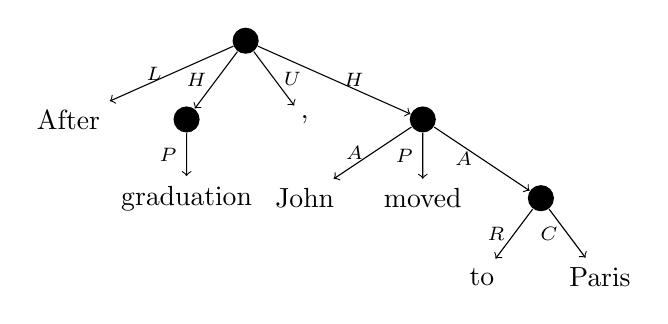
\begin{tikzpicture}[level distance=10mm, ->]
    \node (ROOT) [fill=black, circle] {}
      child {node (After) {After} edge from parent node[left] {\scriptsize $L$}}
      child {node (graduation) [fill=black, circle] {}
      {
        child {node {graduation} edge from parent node[left] {\scriptsize $P$}}
      } edge from parent node[left] {\scriptsize $H$} }
      child {node {,} edge from parent node[right] {\scriptsize $U$}}
      child {node (moved) [fill=black, circle] {}
      {
        child {node (John) {John} edge from parent node[left] {\scriptsize $A$}}
        child {node {moved} edge from parent node[left] {\scriptsize $P$}}
        child {node [fill=black, circle] {}
        {
          child {node {to} edge from parent node[left] {\scriptsize $R$}}
          child {node {Paris} edge from parent node[left] {\scriptsize $C$}}
        } edge from parent node[left] {\scriptsize $A$} }
      } edge from parent node[right] {\scriptsize $H$} }
      ;
  \end{tikzpicture}
  \caption{Tree approximation for the UCCA graph in \figref{main:fig:graduation} in the paper}
  \label{fig:con_example}
\end{figure}

To convert a UCCA graph to a bilexical tree, we first convert it to a bilexical graph, and then
remove the remote edges.
The corresponding dependency tree is given in \figref{fig:dep_example}.

\begin{figure}[H]
\centering
\begin{dependency}[theme = simple]
\begin{deptext}[column sep=.7em,ampersand replacement=\^]
After \^ graduation \^ , \^ John \^ moved \^ to \^ Paris \\
\end{deptext}
\depedge{2}{1}{L}
\depedge{2}{3}{U}
\depedge{5}{4}{A}
\depedge{2}{5}{H}
\depedge{7}{6}{R}
\depedge{5}{7}{A}
\end{dependency}
  \caption{Bilexical tree approximation for the UCCA graph in \figref{main:fig:graduation} in the paper}
  \label{fig:dep_example}
\end{figure}

\paragraph{Tree approximation-based out-of-domain results.}

The scores in \tabref{tab:ood_converted} were obtained on primary edges when running the
tree approximation parsers on the out-of-domain data set (\textit{20K Leagues}).
Scores on remote edges are zero, since they are not reconstructed by the conversion.
\begin{table}[H]
  \centering
\begin{tabular}{l|ccc}
& \textbf{LP} & \textbf{LR} & \textbf{LF} \\
\hline
\multicolumn{4}{l}{\rule{0pt}{2ex} \footnotesize Constituency Tree Conversion} \\
\textsc{uparse} & 57 & 59.4 & 58 \\
Upper Bound & 100 & 100 & 100 \\
\hline
\multicolumn{4}{l}{\rule{0pt}{4ex} \footnotesize Dependency Tree Conversion} \\
Malt$_{\textrm{arc-standard}}$ & 62.3 & 55.9 & 58.7 \\
Malt$_{\textrm{arc-eager}}$ & 62.8 & 56.3 & 59.2 \\
LSTM & {\bf 70.1} & {\bf 63.3} & {\bf 66.1} \\
Upper Bound & 93.5 & 82.5 & 87.6 \\
\end{tabular}
\caption{Results for tree approximation-based parsing when tested on out-of-domain data
(\textit{20K Leagues})}
\label{tab:ood_converted}
\end{table}

\section{Feature templates for sparse linear classifier}

\figref{fig:features} presents the feature templates used by the perceptron-based parser.
All feature templates define binary features.
For some of the features, we used the notion of \textit{head word},
defined by the $h^*$ function (\secref{sec:conversion}).
While head words are not explicitly represented in the UCCA scheme, these
features proved useful as means of encoding word-to-word relations.

\begin{figure}[h]
\centering
\begin{adjustbox}{margin=3pt,frame}
\begin{tabular}{l}
{\footnotesize Features from \cite{zhang2009transition}:} \\
\textbf{unigrams} \\
$s_0te, s_0we, s_1te, s_1we, s_2te, s_2we, s_3te, s_3we,$ \\
$b_0wt, b_1wt, b_2wt, b_3wt,$ \\
$s_0lwe, s_0rwe, s_0uwe, s_1lwe, s_1rwe, s_1uwe$ \\
\textbf{bigrams} \\
$s_0ws_1w, s_0ws_1e, s_0es_1w, s_0es_1e, s_0wb_0w, s_0wb_0t,$ \\
$s_0eb_0w, s_0eb_0t, s_1wb_0w, s_1wb_0t, s_1eb_0w, s_1eb_0t,$ \\
$b_0wb_1w, b_0wb_1t, b_0tb_1w, b_0tb_1t$ \\
\textbf{trigrams} \\
$s_0es_1es_2w, s_0es_1es_2e, s_0es_1eb_0w, s_0es_1eb_0t,$ \\
$s_0es_1wb_0w, s_0es_1wb_0t, s_0ws_1es_2e, s_0ws_1eb_0t$ \\
\textbf{separator} \\
$s_0wp, s_0wep, s_0wq, s_0wcq, s_0es_1ep, s_0es_1eq,$ \\
$s_1wp, s_1wep, s_1wq, s_1weq$ \\

\textbf{extended} \footnotesize \cite{zhu2013fast} \\
$s_0llwe, s_0lrwe, s_0luwe, s_0rlwe, s_0rrwe,$ \\
$s_0ruwe, s_0ulwe, s_0urwe, s_0uuwe, s_1llwe,$ \\
$s_1lrwe, s_1luwe, s_1rlwe, s_1rrwe, s_1ruwe$ \\
\end{tabular}
\begin{tabular}{l}
\textbf{disco} \footnotesize \cite{maier2015discontinuous} \\
$s_0xwe, s_1xwe, s_2xwe, s_3xwe,$ \\
$s_0xte, s_1xte, s_2xte, s_3xte,$ \\
$s_0xy, s_1xy, s_2xy, s_3xy$ \\
$s_0xs_1e, s_0xs_1w, s_0xs_1x, s_0ws_1x, s_0es_1x,$ \\
$s_0xs_2e, s_0xs_2w, s_0xs_2x, s_0ws_2x, s_0es_2x,$ \\
$s_0ys_1y, s_0ys_2y, s_0xb_0t, s_0xb_0w$ \\

{\footnotesize Features from \cite{tokgoz2015transition}:} \\
\textbf{counts} \\
$s_0P, s_0C, s_0wP, s_0wC, b_0P, b_0C, b_0wP, b_0wC$ \\
\textbf{edges} \\
$s_0s_1, s_1s_0, s_0b_0, b_0s_0, s_0b_0e, b_0s_0e$ \\
\textbf{history} \\
$a_0, a_1$ \\

\textbf{remote} \footnotesize (Novel, UCCA-specific features) \\
$s_0R, s_0wR, b_0R, b_0wR$
\end{tabular}
\end{adjustbox}
\captionsetup{singlelinecheck=off}
\caption[]{\label{fig:features}
  Binary feature templates for \parser{sparse}. Notation:
  \begin{itemize}
  \item $s_i$, $b_i$: $i$th stack and buffer items.
  \item $w$, $t$: word form and POS tag of the terminal returned by $h^*(\cdot)$
  (\secref{sec:conversion}).
  \item $e$: edge label to the node returned by $h(\cdot)$.
  \item $l$, $r$ ($ll$, $rr$): leftmost and rightmost (grand)children.
  \item $u$ ($uu$): unary (grand)child, when only one exists.
  \item $p$: unique separator punctuation between $s_0$ and $s_1$. $q$: separator count.
  \item $x$: gap type (``none'', ``pass'' or ``gap'') at the sub-graph under the current node.
  \item $y$: sum of gap lengths \protect\cite{Maier:Lichte:11}.
  \item $P$, $C$: number of parents and children.
  \item $R$: number of remote children.
  \item $a_i$: action taken $i$ steps back.
  \end{itemize}
}
\end{figure}

\paragraph{Feature ablation experimental results.}

The following results, in percents,
were obtained on the development set in the feature ablation experiment
(\secref{main:sec:results} in the paper).
The first row corresponds to \parser{sparse} as in the main experiment.
In each of the other rows, one feature set is excluded.
Columns are the same as in \tabref{main:table:results} in the paper.
  
\begin{table}[H]
\centering
\begin{tabular}{l|ccc|ccc}
& \multicolumn{3}{c|}{Primary} & \multicolumn{3}{c}{Remote} \\
& \textbf{LP} & \textbf{LR} & \textbf{LF} & \textbf{LP} & \textbf{LR} & \textbf{LF} \\
\hline
\parser{sparse} & 62.6	& 55.7 & 58.9 & 20 & 12.9 & 15.7 \\
\parser{sparse}$-$\textbf{unigrams} & 62.5 & 52.6 & 57.1 & 18.9 & 10.1 & 13.2 \\
\parser{sparse}$-$\textbf{bigrams} & 59.8 & 50.0 & 54.4 & 18.2 & 12.2 & 14.6 \\
\parser{sparse}$-$\textbf{trigrams} & 63.7 & 55.0 & 59.0 & 20.7 & 12.0 & 15.2 \\
\parser{sparse}$-$\textbf{separator} & 62.9 & 53.5 & 57.8 & 17.8 & 11.7 & 14.1 \\
\parser{sparse}$-$\textbf{extended} & 62.9 & 52.8 & 57.4 & 17.4 & 11.5 & 13.9 \\
\parser{sparse}$-$\textbf{disco} & 63.6 & 53.6 & 58.2 & 19.7 & 11.5 & 14.5 \\
\parser{sparse}$-$\textbf{counts} & 63.3 & 52.8 & 57.6 & 14.6 & 10.6 & 12.3 \\
\parser{sparse}$-$\textbf{edges} & 63.5 & 54.9 & 58.9 & 23.6 & 14.5 & 17.9 \\
\parser{sparse}$-$\textbf{history} & 63.1 & 53.2 & 57.8 & 23.7 & 14.5 & 18.0 \\
\parser{sparse}$-$\textbf{remote} & 63.5 & 53.2 & 57.9 & 17.2 & 10.6 & 13.1 \\
\parser{sparse}$-$\textbf{ratio} & 63.7 & 48.3 & 55.0 & 25.4 & 13.6 & 17.7
\end{tabular}
\caption{Results for feature ablation experiments on \parser{sparse}.}
\label{tab:ablation}
\end{table}


\section{Extended Presentation of UCCA}

\paragraph{Linkage.}

The following figure demonstrates a linkage relation, omitted from \figref{main:fig:graduation}
in the paper.

\begin{figure}[h]
  \centering
  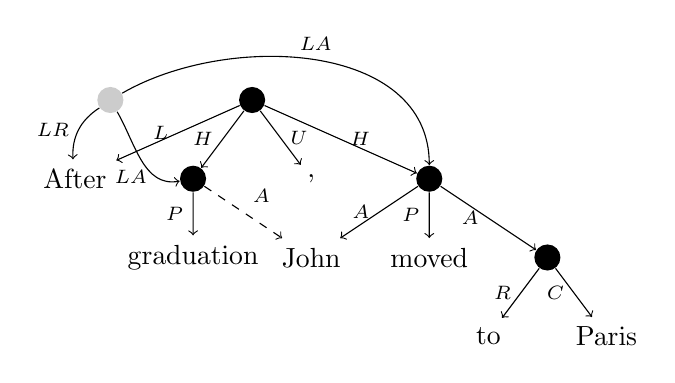
\begin{tikzpicture}[level distance=10mm, ->]
    \node (ROOT) [fill=black, circle] {}
      child {node (After) {After} edge from parent node[left] {\scriptsize $L$}}
      child {node (graduation) [fill=black, circle] {}
      {
        child {node {graduation} edge from parent node[left] {\scriptsize $P$}}
      } edge from parent node[left] {\scriptsize $H$} }
      child {node {,} edge from parent node[right] {\scriptsize $U$}}
      child {node (moved) [fill=black, circle] {}
      {
        child {node (John) {John} edge from parent node[left] {\scriptsize $A$}}
        child {node {moved} edge from parent node[left] {\scriptsize $P$}}
        child {node [fill=black, circle] {}
        {
          child {node {to} edge from parent node[left] {\scriptsize $R$}}
          child {node {Paris} edge from parent node[left] {\scriptsize $C$}}
        } edge from parent node[left] {\scriptsize $A$} }
      } edge from parent node[right] {\scriptsize $H$} }
      ;
    \draw[dashed,->] (graduation) to node [auto] {\scriptsize $A$} (John);
    \node (LKG) at (-1.8,0) [fill=black!20, circle] {};
          \draw[bend right] (LKG) to node [auto, left] {\scriptsize $LR$} (After);
          \draw (LKG) to[out=-60, in=190] node [below] {\scriptsize $LA\quad$} (graduation);
          \draw (LKG) to[out=30, in=90] node [above] {\scriptsize $LA$} (moved);
  \end{tikzpicture}
  \caption{UCCA example with linkage.}
\end{figure}

The linkage relation is represented by the gray node.
$LA$ is \emph{link argument}, and $LR$ is \emph{link relation}.
The relation represents the fact that the \emph{linker} ``After'' links the two parallel scenes
that are the arguments of the linkage.
Linkage relations are another source of multiple parents for a node, which we do not yet handle
in parsing and evaluation.

\paragraph{Implicit units.}

UCCA graphs may contain implicit units with no correspondent in the text.
The following figure shows the annotation for the sentence
``A similar technique is almost impossible to apply to other crops, such as cotton, soybeans and rice.''.
The sentence was used by \cite{oepen2015semeval} to compare between different semantic
dependency schemes.
It includes a single Scene, whose main relation is ``apply'', a secondary relation ``almost impossible'', as well as two complex arguments: ``a similar technique'' and the coordinated argument ``such as cotton, soybeans, and rice.''
In addition, the scenes includes an implicit argument, which represents the agent of the
``apply'' relation.

The parsing of these units is deferred to future work, as it is likely to require different methods
than those explored in this paper \cite{roth2015inducing}.

\begin{figure}[h]
  \centering
  \scalebox{.6}{
  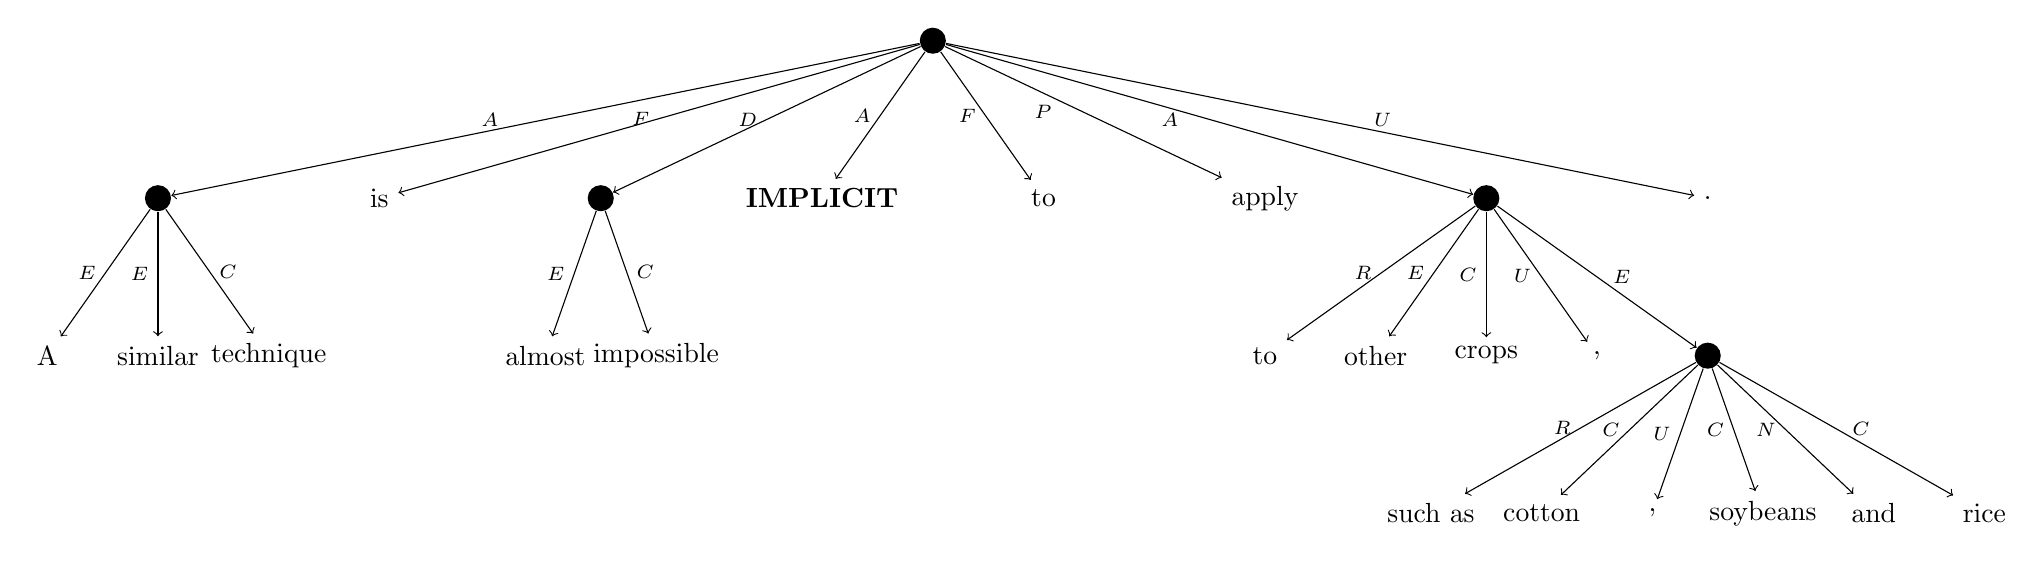
\begin{tikzpicture}[level distance=20mm, ->,
  level 1/.style={sibling distance=8em},
  level 2/.style={sibling distance=4em},
  level 3/.style={sibling distance=4em}]
    \node (ROOT) [fill=black, circle] {}
      child {node [fill=black, circle] {}
      {
        child {node {A} edge from parent node[left] {\scriptsize $E$}}
        child {node {similar} edge from parent node[left] {\scriptsize $E$}}
        child {node {technique} edge from parent node[right] {\scriptsize $C$}}
      } edge from parent node[left] {\scriptsize $A\quad$ \hspace{1mm} } }
      child {node {is} edge from parent node[left] {\scriptsize $F$}}
      child {node [fill=black, circle] {}
      {
        child {node {almost} edge from parent node[left] {\scriptsize $E$}}
        child {node {impossible} edge from parent node[right] {\scriptsize $C$}}
      } edge from parent node[left] {\scriptsize $D$} }
      child {node {\textbf{IMPLICIT}} edge from parent node[left] {\scriptsize $A$}}
      child {node {to} edge from parent node[left] {\scriptsize $F$}}
      child {node {apply} edge from parent node[left] {\scriptsize $P\quad$}}
      child {node [fill=black, circle] {}
      {
        child {node {to} edge from parent node[left] {\scriptsize $R$}}
        child {node {other} edge from parent node[left] {\scriptsize $E$}}
        child {node {crops} edge from parent node[left] {\scriptsize $C$}}
        child {node {,} edge from parent node[left] {\scriptsize $U$}}
        child {node [fill=black, circle] {}
        {
          child {node {such as} edge from parent node[left] {\scriptsize $R$}}
          child {node {cotton} edge from parent node[left] {\scriptsize $C$}}
          child {node {,} edge from parent node[left] {\scriptsize $U$}}
          child {node {soybeans} edge from parent node[left] {\scriptsize $C$}}
          child {node {and} edge from parent node[left] {\scriptsize $N$}}
          child {node {rice} edge from parent node[right] {\scriptsize $\; C$}}
        } edge from parent node[right] {\scriptsize $\; E$ \hspace{1mm} } }
      } edge from parent node[left] {\scriptsize $A\;$ \hspace{1mm} } }
      child {node {.} edge from parent node[right] {\scriptsize $\quad \quad U$}}
      ;
  \end{tikzpicture}
  }
  \caption{UCCA example with an implicit unit.}
\end{figure}

\paragraph{Statistics of Linkage and Implicit Nodes}

\tabref{table:data_linkage_implicit} shows the statistics of linkage and implicit nodes
in the corpora.

\begin{table}[h]
\centering
\begin{tabular}{l|ccc|c}
& \multicolumn{3}{c|}{Wiki} & 20K \\
& \small Train & \small Dev & \small Test & Leagues \\
\hline
nodes \\
\# implicit & 900 & 119 & 80 & 241 \\
\# linkage & 2833 & 241 & 364 & 376 \\
\hline
edges \\
\# linkage & 8853 & 737 & 1105 & 957
\end{tabular}
\caption{Statistics of linkage and implicit nodes in the
\textit{Wiki} and \textit{20K Leagues} UCCA corpora.
Cf. \tabref{main:table:data} in the paper.
}
\label{table:data_linkage_implicit}
\end{table}



\bibliography{references}
\bibliographystyle{eacl2017}

\end{document}
